\documentclass{article}
% PACKAGES %
\usepackage[english]{} % Sets the language
\usepackage[margin=2cm]{geometry} % Sets the margin size
\usepackage{fancyhdr} % Allows creation of headers
\usepackage{xcolor} % Allows the use of color in text
\usepackage{float} % Allows figures and tables to be floats
\usepackage{appendix}
\usepackage{amsmath} % Enhanced math package prepared by the American Mathematical Society
	\DeclareMathOperator{\sech}{sech} % Include sech
\usepackage{amssymb} % AMS symbols package
\usepackage{mathrsfs}% More math symbols
\usepackage{breqn} % Allows line breaking in math mode
\usepackage{cancel} % Allows math strikethroughs to show cancellations
\usepackage{bm} % Allows you to use \bm{} to make any symbol bold
\usepackage{bbold} % Allows more bold characters
\usepackage{verbatim} % Allows you to include code snippets
\usepackage{setspace} % Allows you to change the spacing between lines at different points in the document
\usepackage{parskip} % Allows you alter the spacing between paragraphs
\usepackage{multicol} % Allows text division into multiple columns
\usepackage{units} % Allows fractions to be expressed diagonally instead of vertically
\usepackage{booktabs,multirow,multirow} % Gives extra table functionality
\usepackage[final]{pdfpages} % Allows pdfs to be imported
\usepackage{hyperref} % Allows hyperlinks in the document
\usepackage{rotating} % Allows tables to be rotated
\usepackage{graphicx} % Enhanced package for including graphics/figures
	% Set path to figure image files
	\graphicspath{ {fig/} }
\usepackage{listings} % for including text files
	\lstset{basicstyle=\ttfamily\scriptsize,
        		  keywordstyle=\color{blue}\ttfamily,
        	  	  stringstyle=\color{red}\ttfamily,
          	  commentstyle=\color{gray}\ttfamily,
          	 }		
\newcommand{\tab}{\-\hspace{1cm}}

\newcommand{\p}{\partial}

\newcommand{\Oh}{\hat{\Omega}}
\newcommand{\cur}{\vec{J}}
\newcommand{\pos}{\vec{r}}
\newcommand{\rt}{(\vec{r},t)}
\newcommand{\rOt}{(\vec{r},\Oh,t)}


% Create a header w/ Name & Date
\pagestyle{fancy}
\rhead{\textbf{Mitch Negus} \; 10/6/2017}

\begin{document}
\thispagestyle{empty}

{\bf {\large {NE250 Homework {2} \hfill Mitch Negus\\
		\hspace*{\fill} 10/6/2017\\ }}}
		
%%%%%%%%%%%%%%%%%%%%%%%%%%%%%%%%%% PROBLEM 1 %%%%%%%%%%%%%%%%%%%%%%%%%%%%%%%%%%

\section*{Problem 1}

If the energy distribution for fission neutrons from $^{235}\text{U}$ follows the functional approximation (for energy in MeV)
$$ \chi(E) = 0.453e^{-1.036E}\sinh(\sqrt{2.29E}), $$
then the most probable energy of a neutron corresponds to the maximum of the function. A maximum value will be found at a critical point of the function, which can be found via differentiation (specifically when $\frac{d\chi}{dE} = 0$):
\begin{align*}
\frac{d\chi}{dE}= 0	&= \frac{d}{dE}\left(0.453e^{-1.036E_{\text{max}}}\sinh(\sqrt{2.29E_{\text{max}}})\right) \\
				  0	&= 0.453\frac{d}{dE}\left(e^{-1.036E_{\text{max}}}\sinh(\sqrt{2.29E_{\text{max}}})\right) \\
				  0	&= 0.453\left[e^{-1.036E}\frac{d}{dE}\sinh(\sqrt{2.29E_{\text{max}}})+\frac{d}{dE}\left(e^{-1.036E_{\text{max}}}\right)\sinh(\sqrt{2.29E_{\text{max}}})\right] \\
				  0	&= 0.453\left[e^{-1.036E}\cosh(\sqrt{2.29E})\frac{d}{dE}\left(\sqrt{2.29E_{\text{max}}}\right)-1.036e^{-1.036E}\sinh(\sqrt{2.29E})\right] \\
				  0	&= 0.453\left[e^{-1.036E}\cosh(\sqrt{2.29E})\frac{\sqrt{2.29}}{2\sqrt{E_{\text{max}}}}-1.036e^{-1.036E}\sinh(\sqrt{2.29E})\right] \\
				  0	&= \frac{\sqrt{2.29}\cosh(\sqrt{2.29E})}{2\sqrt{E_{\text{max}}}}-1.036\sinh(\sqrt{2.29E}) \\
				  0	&= 1 - 1.369\sqrt{E_{\text{max}}}\tanh(\sqrt{2.29E_{\text{max}}}) \\
				  1	&= 1.369\sqrt{E_{\text{max}}}\tanh(\sqrt{2.29E_{\text{max}}}) \\
\end{align*}
$$\boxed{ E_{\text{max}}= 0.724\text{ MeV} }$$

The average energy can be found by finding the expected value of the function on the domain $[0,\infty)$.
\begin{align*}
E_{\text{ave}}	&= \int_0^{\infty} E\,\chi(E)\,dE \\
				&= \int_0^{\infty} E\left(0.453e^{-1.036E}\sinh(\sqrt{2.29E})\right)\,dE \\
				&= 0.453\int_0^{\infty} E\,e^{-1.036E}\sinh(\sqrt{2.29E})\,dE \\
\end{align*}
This integral cannot be solved analytically. Solving numerically (with Wolram Alpha),
$$\boxed{ E_{\text{ave}} = 1.98\text{ MeV} }$$



\newpage
%%%%%%%%%%%%%%%%%%%%%%%%%%%%%%%%%% PROBLEM 2 %%%%%%%%%%%%%%%%%%%%%%%%%%%%%%%%%%

\section*{Problem 2}

A general reaction rate for process $x$ as a function of energy can be defined as 
$$ R_x(E) = \Sigma_x(E) \phi(E) $$
where $\Sigma_x(E)$ is the macroscopic cross section for reaction $x$ and $\phi$ is the neutron flux, both at energy $E$. The macroscopic cross section can be further decomposed, so that
$$ R_x(E) = n_x \sigma_x(E) \phi(E) .$$
Comparing neutron-neutron reactions with all neutron-nuclei reactions, the ratio of reaction rates is
$$ \frac{R_{nn}(E)}{R_{tot}(E)} = \frac{n_n \sigma_{nn}(E) \phi(E)}{n_{\text{UO}_2} \sigma_{tot}(E) \phi(E)} .$$

We can know that the neutron flux is $\phi(0.025\text{ eV} = 10^{16}\text{ neutrons/(cm}^2\cdot\text{s)}$ and they are at thermal energies ($E = 0.025$ eV and traveling at $v = \sqrt{\frac{2(0.025\text{\tiny eV})}{m_n}} = 2.190\times10^5\text{ cm/s}$). The neutrons that are then in a 1 cm$^3$ volume at any given second is
$$ n_n = \frac{\phi(0.025\text{ eV})}{v} = \frac{10^{16}\text{ neutrons/(cm}^2\cdot\text{s)}}{2.190\times10^5\text{ cm/s}} = 4.566\times10^{10}\text{ neutrons/cm}^3 $$

For UO$_2$, $\rho = 10.97\text{ g/cm}^3$, $m_{\text{O}} = 16.0\text{ g/mol}$, $m_{\text{U}8} = 238.05\text{ g/mol}$, and $m_{\text{U}5} = 235.04\text{ g/mol}$. If we use an enrichment of 5\% (atom percent), then $m_{\text{UO}_2} = 0.95(238.05) + 0.05(235.04) + 2(16.0) = 269.90$ g/mol. For number density, we find
$$ n_{\text{UO}_2} = \frac{\rho N_A}{m_{\text{UO}_2}} = \frac{(10.97\text{ g/cm}^3)(6.022\times10^{23})}{269.90\text{ g/mol}} = 2.448\times10^{22}\text{ molecules/cm}^3$$

Additionally, we're given that $\sigma_{nn} = 10$ b, and we can determine the microscopic cross section for UO$_2$ from tabulated data. (From ENDF/B-VII.1 at 0.025 eV: $\sigma_{tot,\text{U}8} = 11.962\text{ b},\sigma_{tot,\text{U}5} = 698.856\text{ b}, \text{ and } \sigma_{tot,\text{O}} = 3.852\text{ b}$)
$$ \sigma_{tot} = 0.95\sigma_{tot,\text{U}8} + 0.05\sigma_{tot,\text{U}5} + 2\sigma_{tot,\text{O}} $$
$$ \sigma_{tot} = 0.95(11.962\text{ b}) + 0.05(698.856\text{ b}) + 2(3.852\text{ b}) $$
$$ \sigma_{tot} = 54.011\text{ b} $$

We can now sove for the ratio of reaction rates (noting that $\phi(E)$ cancels in the numerator and denominator)

$$ \frac{R_{nn}(E)}{R_{tot}(E)} = \frac{n_n \sigma_{nn}(E)}{n_{\text{UO}_2} \sigma_{tot}(E)} = \frac{(4.566\times10^{10}\text{ neutrons/cm}^3)(10\text{ b})}{(2.448\times10^{22}\text{ molecules/cm}^3)(54.011\text{ b})}$$
$$ \frac{R_{nn}(E)}{R_{tot}(E)} = 3.40\times10^{-13} $$
The rate of neutron-neutron collisions is \underline{13 orders of magnitudes less} than the rate of neutron-UO$_2$ collisions.



\newpage
%%%%%%%%%%%%%%%%%%%%%%%%%%%%%%%%%% PROBLEM 3 %%%%%%%%%%%%%%%%%%%%%%%%%%%%%%%%%%

\section*{Problem 3}



%%%%%%%%%%%%%%%%%%%%%%%%%%%%%%%%%% PROBLEM 4 %%%%%%%%%%%%%%%%%%%%%%%%%%%%%%%%%%

\section*{Problem 4}

First, we define the average scattering cosine $\bar{\mu}_0$ as the average dot product, $\langle \Oh \cdot \Oh' \rangle$. When normalized by $4\pi\Sigma_s$, the total of cross sections for scattering from any angle $\Oh$ to any other angle $\Oh'$, this is
$$ \bar{\mu}_0 \equiv \langle \Oh \cdot \Oh' \rangle = \left(\frac{1}{4\pi\Sigma_s}\right)  \int_{4\pi} d\Oh \int_{4\pi} d\Oh' \, \Oh \cdot \Oh' \Sigma_s(\Oh \cdot \Oh') $$

In the center of mass system, the probability that a particle scatters in any direction is roughly uniform, $\Sigma_{\text{CM}}(\theta_C) = \frac{\Sigma_s}{4\pi}$,
$$ \bar{\mu}_0 = \frac{1}{\Sigma_s}  \int_{4\pi} d\Oh \int_{4\pi} d\Oh' \, \Oh \cdot \Oh' \Sigma_{\text{CM}}(\theta_C) .$$



\newpage
%%%%%%%%%%%%%%%%%%%%%%%%%%%%%%%%%% PROBLEM 5 %%%%%%%%%%%%%%%%%%%%%%%%%%%%%%%%%%

\section*{Problem 5}

A critical reactor has a multiplication factor of $k=1$. The multiplication factor (for an infinite reactor) can be defined as
$$ k_{\infty} \equiv \frac{\text{\# neutrons produced}}{\text{\# neutrons absorbed}} $$
Mathematically, the number of neutrons produced is $\int_0^{\infty} \nu \Sigma_f(E)\phi(E)\,dE$ and the number of neutrons absorbed is $\int_0^{\infty} \Sigma_a(E)\phi(E)\,dE$. Altogether, we can mathematically describe a critical reactor as 
$$ 1 = \frac{\int_0^{\infty} \nu \Sigma_f(E)\phi(E)\,dE}{\int_0^{\infty} \Sigma_a(E)\phi(E)\,dE} $$
or equivalently
$$ \int_0^{\infty} \nu \Sigma_f(E)\phi(E)\,dE = \int_0^{\infty} \Sigma_a(E)\phi(E)\,dE. $$
Since we are considering only thermal cross sections, we will let $\Sigma_X(E) = \Sigma_X(0.025\text{ eV}) = \Sigma_{X,T}$ and we find
$$ \nu \Sigma_{f,T} \int_0^{\infty} \phi(E)\,dE = \Sigma_{a,T} \int_0^{\infty} \phi(E)\,dE. $$
The integrals over flux cancel, and so
$$ \nu \Sigma_{f,T} = \Sigma_{a,T} .$$
The macroscopic cross sections can be rewritten as $\Sigma_{f,T} = \Sigma_{f,T,\text{f}}$ and $\Sigma_{a,T} = \Sigma_{a,T,\text{f}} + \Sigma_{a,T,\text{m}}$ where subscripts $\text{f}$ and $\text{m}$ denote fuel and moderator, respectively. Furthermore, each macroscopic cross section for each material can be expressed in terms of the material's number density and microscopic cross section, $\Sigma = n\sigma$. In total
$$ \nu n_{\text{f}} \sigma_{f,T,\text{f}} = n_{\text{f}} \sigma_{a,T,\text{f}} + n_{\text{m}} \sigma_{a,T,\text{m}} .$$
The fuel-to-moderator density at criticality can then be expressed as
$$ \frac{n_{\text{f}}}{n_{\text{m}}} = \frac{\sigma_{a,T,\text{m}}}{\nu \sigma_{f,T,\text{f}} - \sigma_{a,T,\text{f}}} .$$
\-\\

\begin{multicols}{4}
\subsection*{\textit{a.}) \normalsize Graphite}
$$ \frac{n_{\text{f}}}{n_{\text{m}}} = 4.55\times10^{-6}$$

\subsection*{\textit{b.}) \normalsize Beryllium}
$$ \frac{n_{\text{f}}}{n_{\text{m}}} = 1.36\times10^{-5}$$

\subsection*{\textit{c.}) \normalsize Water}
$$ \frac{n_{\text{f}}}{n_{\text{m}}} = 8.99\times10^{-4}$$

\subsection*{\textit{d.}) \normalsize Graphite}
$$ \frac{n_{\text{f}}}{n_{\text{m}}} = 1.64\times10^{-6}$$
\end{multicols}

\-\\
(see attached Jupyter notebook for full calculations)



\newpage
%%%%%%%%%%%%%%%%%%%%%%%%%%%%%%%%%% PROBLEM 6 %%%%%%%%%%%%%%%%%%%%%%%%%%%%%%%%%%

\section*{Problem 6}

\subsection*{\textit{a.})}

Like in Problem 5, 
$$k_{\infty} = \frac{\int_0^{\infty} \nu \Sigma_f(E)\phi(E)\,dE}{\int_0^{\infty} \Sigma_a(E)\phi(E)\,dE} .$$
Again, since we are only considering cross sections averaged over the fast spectrum, we can state that $\Sigma_X(E) = \Sigma_{X,F},$ and then 
$$ k_{\infty} = \frac{\nu \Sigma_{f,F} \int_0^{\infty} \phi(E)\,dE}{\Sigma_{a,F} \int_0^{\infty} \phi(E)\,dE} = \frac{\nu \Sigma_{f,F}}{\Sigma_{a,F}}.$$
Next, we repeat our decomposition of the numerator and denominator, leaving 
$$ k_{\infty} = \frac{\nu_{\text{PuO}_2} n_{\text{PuO}_2} \sigma_{F,\text{PuO}_2} + \nu_{\text{UO}_2} n_{\text{UO}_2} \sigma_{F,\text{UO}_2}}{n_{\text{PuO}_2} \sigma_{a,F,\text{PuO}_2} + n_{\text{UO}_2} \sigma_{a,F,\text{UO}_2} + n_{\text{Fe}} \sigma_{a,F,\text{Fe}} + n_{\text{Na}} \sigma_{a,F,\text{Na}}} $$

After solving this equation with the given values, we find
$$\boxed{ k_{\infty} = 1.332 }$$


\subsection*{\textit{b.})}

We can use the densities and volume fractions to determine the fraction of the core mass that is fuel. 
$$\boxed{ 61.6\% \text{ is fuel} }$$


\subsection*{\textit{c.})}

If $k = 1$ and the non-leakage probability is $P_{NL} = 0.90$, then we can reexpress our earlier equation as

$$ k = 1 = P_{NL}\frac{\nu \Sigma_{f,F} \int_0^{\infty} \phi(E)\,dE}{\Sigma_{a,F} \int_0^{\infty} \phi(E)\,dE} = P_{NL}\frac{\nu \Sigma_{f,F}}{\Sigma_{a,F}},$$

or 

$$ P_{NL}\nu \Sigma_{f,F} = \Sigma_{a,F}. $$

When separated into individual materials, this is 

$$ P_{NL}\sum_i \nu_i n_i \sigma_{f,i} = \sum_j n_j \sigma_{a,j} .$$

or explicitly

$$ P_{NL} \left( \nu_{\text{PuO}_2} n_{\text{PuO}_2} \sigma_{F,\text{PuO}_2} + \nu_{\text{UO}_2} n_{\text{UO}_2} \sigma_{F,\text{UO}_2}\right) = n_{\text{PuO}_2} \sigma_{a,F,\text{PuO}_2} + n_{\text{UO}_2} \sigma_{a,F,\text{UO}_2} + n_{\text{Fe}} \sigma_{a,F,\text{Fe}} + n_{\text{Na}} \sigma_{a,F,\text{Na}} $$

We recall that $n_{\text{PuO}_2} = f_{\text{f,PuO}_2}(0.3)\frac{\rho_{\text{PuO}_2} N_A}{m_{\text{PuO}_2}}$ and $n_{\text{UO}_2} = (1-f_{\text{f,PuO}_2})(0.3)\frac{\rho_{\text{UO}2} N_A}{m_{\text{UO}_2}}$, while $n_{\text{Na}} = (0.5)\frac{\rho_{\text{Na}} N_A}{m_{\text{Na}}}$and $n_{\text{Fe}} = (0.2)\frac{\rho_{\text{Fe}} N_A}{m_{\text{Fe}}}$. We can substitute these expressions into the equation above and solve for $f_{\text{f,PuO}_2}$. 

$$\boxed{ \text{The fuel must be } 10.322\% \text{ PuO}_2 \text{ and } 89.678\% \text{ UO}_2 \text{ for a critical reactor with } P_{NL} = 0.9 }$$

(see attached Jupyter notebook for full calculations)



%%%%%%%%%%%%%%%%%%%%%%%%%%%%%%%%%% PROBLEM 7 %%%%%%%%%%%%%%%%%%%%%%%%%%%%%%%%%%

\section*{Problem 7}

We are told that the albedo is defined as the ratio of current out of a reflecting surface and into a reflecting surface, $\alpha \equiv \frac{J_{\text{out}}}{J_{\text{in}}}$. We also note that without an internal source, the one-speed, one-dimensional diffusion equation in the reflector is given by
$$ \frac{d^2\phi(x)}{dx} - \frac{1}{L^2}\phi(x) = 0 $$
where $L = \sqrt{\frac{D}{\Sigma_a}}$ is the diffusion length in the reflector and $D$ is the diffusion coefficient of the reflector (both constant).

This equation is constrained by two boundary conditions: 
$$ \phi(\tilde{a}) = 0 $$
$$ J_+(0) = J_{\text{in}} .$$
The first of these states that the flux must go to zero at the extrapolated distance (no infinite flux over all space), and the second implies that the uniformly distributed slab source can be treated as a uniform plane source at the boundary from the perspective of the reflector.

We can now solve the one-speed diffusion equation for the reflector. The solution is of the form
$$ \phi(x) = C_1 e^{x/L} + C_2 e^{-x/L} .$$
Applying our first boundary condition,
$$ \phi(\tilde{a}) = 0 = C_1 e^{\tilde{a}/L} + C_2 e^{-\tilde{a}/L} $$
$$ C_2 = -C_1 e^{2\tilde{a}/L} $$
and so
$$ \phi(x) = C_1 e^{x/L} - C_1 e^{2\tilde{a}/L} e^{-x/L}, $$
or, when factoring out $C = 2 C_1 e^{\tilde{a}/L}$
$$ \phi(x) = C \frac{e^{(x-\tilde{a})/L} -  e^{(\tilde{a}-x)/L}}{2} = C \sinh\left(\frac{x-\tilde{a}}{L}\right). $$
We can then apply our second boundary condition if we note that 
$$ J_+(x) = \frac{\phi(x)}{4} - \frac{D}{2}\frac{d\phi(x)}{dx} $$
which means
$$ J_{\text{in}} = \frac{C \sinh\left(\frac{-\tilde{a}}{L}\right)}{4} - \frac{D}{2} \frac{d}{dx}\left[ C \sinh\left(\frac{x-\tilde{a}}{L}\right) \right]_{x=0} $$
or more simply
$$ J_{\text{in}} = \frac{C\sinh\left(\frac{-\tilde{a}}{L}\right)}{4} - \frac{CD}{2L}\cosh\left(\frac{-\tilde{a}}{L}\right) $$
We also know that $J(x) = -D\frac{d\phi(x)}{dx}$, so
\begin{align*}
 J(x)	&= -D \frac{d}{dx} \left[ C \sinh\left(\frac{x-\tilde{a}}{L}\right) \right]\\
 		&= -\frac{CD}{L} \cosh\left(\frac{x-\tilde{a}}{L}\right)
\end{align*}
Finally,  since $J(x) = J_+(x) - J_-(x)$,
$$ J(0) = J_+(0) - J_-(0) = J_{\text{in}}-J_{\text{out}} $$
or equivalently,
\begin{align*}
J_{\text{out}}	&= J_{\text{in}} - J(0) \\
				&= \frac{C\sinh\left(\frac{-\tilde{a}}{L}\right)}{4} - \frac{CD}{2L}\cosh\left(\frac{-\tilde{a}}{L}\right) +\frac{CD}{L} \cosh\left(\frac{-\tilde{a}}{L}\right) \\
				&= \frac{C\sinh\left(\frac{-\tilde{a}}{L}\right)}{4} + \frac{CD}{2L}\cosh\left(\frac{-\tilde{a}}{L}\right) 
\end{align*}
Altogether, we have
\begin{align*}
\frac{J_{\text{out}}}{J_{\text{in}}}	&= \frac{\frac{C\sinh\left(\frac{-\tilde{a}}{L}\right)}{4} + \frac{CD}{2L}\cosh\left(\frac{-\tilde{a}}{L}\right)}{\frac{C\sinh\left(\frac{-\tilde{a}}{L}\right)}{4} - \frac{CD}{2L}\cosh\left(\frac{-\tilde{a}}{L}\right)} \\
										&= \frac{1 + \frac{2D}{L}\coth\left(\frac{-\tilde{a}}{L}\right)}{1 - \frac{2D}{L}\coth\left(\frac{-\tilde{a}}{L}\right)} 
\end{align*}
Since hyperbolic cotangent is an odd function, we can simplify this to
$$\boxed{\alpha = \frac{1 - \frac{2D}{L}\coth\left(\frac{\tilde{a}}{L}\right)}{1 + \frac{2D}{L}\coth\left(\frac{\tilde{a}}{L}\right)} }$$ 



%%%%%%%%%%%%%%%%%%%%%%%%%%%%%%%%%% PROBLEM 8 %%%%%%%%%%%%%%%%%%%%%%%%%%%%%%%%%%

\section*{Problem 8}

From the previous problem, $\alpha \equiv \frac{J_{\text{out}}}{J_{\text{in}}}$. If we further define $\beta \equiv \frac{J_+(a)-J_-(a)}{J_+(a)}$, we can express $\beta$ in terms of $\alpha$ through algebraic maniupulation. First, we let $J_+(a) = J_{\text{in}}$ and $J_-(a) = J_{\text{out}}$ for the right handed boundary.
\begin{align*}
\beta	&= \frac{J_{\text{in}}-J_{\text{out}}}{J_{\text{in}}} \\
		&= 1 - \frac{J_{\text{out}}}{J_{\text{in}}} \\
\boxed{ \beta = 1 - \alpha }
\end{align*}
We can also define $\gamma \equiv \frac{J(a)}{\phi(a)}$ and then express it in terms of $\alpha$ as well. Again we let $J_+(a) = J_{\text{in}}$ and $J_-(a) = J_{\text{out}}$ for the right handed boundary, but we also now note that $J_+(x) = \frac{\phi(x)}{4} - \frac{D}{2}\frac{d\phi(x)}{dx} = \frac{\phi(x)}{4} + \frac{J(x)}{2}$. From here, $\phi(x)$ can be found as $\phi(x) = 4J_-(x) - 2J(x)$. 
\begin{align*}
\gamma	&= \frac{J_+(a)-J_-(a)}{4J_+(a) - 2J(a)} \\
		&= \frac{J_+(a)-J_-(a)}{4J_+(a) - 2J_+(a) + 2J_-(a)} \\
		&= \frac{J_{\text{in}}-J_{\text{out}}}{4J_{\text{in}} - 2J_{\text{in}} + 2J_{\text{out}}} \\
				&= \frac{J_{\text{in}}-J_{\text{out}}}{2(J_{\text{in}} + J_{\text{out}})} \\				
				&= \frac{1-\frac{J_{\text{out}}}{J_{\text{in}}}}{2(1 + \frac{J_{\text{out}}}{J_{\text{in}}})} \\
\boxed{ \gamma = \frac{1 - \alpha}{2(1 + \alpha)} }
\end{align*}

With these values we can then solve for $\alpha$ in terms of each $\beta$ and $\gamma$. Very simply
$$\boxed{ \alpha = 1 - \beta }$$
but also
$$ \gamma = \frac{1 - \alpha}{2(1 + \alpha)} $$
$$ 2\gamma = \frac{1 - \alpha}{1 + \alpha} $$
$$ 2\gamma(1+\alpha) = 1 - \alpha $$
$$ 2\gamma + 2\alpha\gamma = 1 - \alpha $$
$$ 2\gamma - 1 = -\alpha - 2\alpha\gamma $$
$$ 2\gamma - 1 = \alpha(-1 - 2\gamma) $$
$$ \alpha = \frac{2\gamma - 1}{-1 - 2\gamma} $$
$$\boxed{ \alpha = \frac{1-2\gamma}{1+2\gamma} }$$



%%%%%%%%%%%%%%%%%%%%%%%%%%%%%%%%%% PROBLEM 9 %%%%%%%%%%%%%%%%%%%%%%%%%%%%%%%%%%

\section*{Problem 9}

The one-speed diffusion equation for a finite slab containing a uniformly distributed neutron source is 
$$ -D\frac{d^2\phi(x)}{dx^2} + \Sigma_a\phi(x) = s $$
or equivalently (when $L = \sqrt{\frac{D}{\Sigma_a}}$),
$$ \frac{d^2\phi(x)}{dx^2} - \frac{1}{L^2}\phi(x) = -\frac{s}{D} $$
We know that the homogeneous solution to this equation (solving for $\phi(x)$ when $\frac{d\phi(x)}{dx} - \frac{1}{L^2}\phi(x) = 0$) is of the form
$$ \phi(x) = C_1e^{x/L} + C_2e^{-x/L} $$
Next we vary the parameters to solve for the particular solution,
$$ \phi_p(x) = c_1(x)e^{x/L} + c_2(x)e^{-x/L} .$$
Then,
$$ \frac{d\phi_p(x)}{dx} = c_1'(x)e^{x/L} + c_2'(x)e^{-x/L} + \frac{c_1(x)}{L}e^{x/L} - \frac{c_2(x)}{L}e^{-x/L}, $$
however we note that $c_1'(x)e^{x/L} + c_2'(x)e^{-x/L} = 0$ and 
$$ \frac{d\phi_p(x)}{dx} = \frac{c_1(x)}{L}e^{x/L} - \frac{c_2(x)}{L}e^{-x/L}. $$
Taking the second derivative of $\phi(x)$, we have
$$ \frac{d^2\phi_p(x)}{dx^2} = \frac{c_1'(x)}{L}e^{x/L} - \frac{c_2'(x)}{L}e^{-x/L} + \frac{c_1(x)}{L^2}e^{x/L} + \frac{c_2(x)}{L^2}e^{-x/L}. $$
If we plug $\phi_p(x)$ and its second derivative into our original equation, we find
$$ \frac{d^2\phi(x)}{dx^2} - \frac{1}{L^2}\phi(x) = -\frac{s}{D} $$
$$ \frac{c_1'(x)}{L}e^{x/L} - \frac{c_2'(x)}{L}e^{-x/L} + \frac{c_1(x)}{L^2}e^{x/L} + \frac{c_2(x)}{L^2}e^{-x/L} - \frac{1}{L^2}\left(c_1(x)e^{x/L} + c_2(x)e^{-x/L}\right) = -\frac{s}{D} $$
$$ \left(\frac{c_1'(x)}{L}e^{x/L} - \frac{c_2'(x)}{L}e^{-x/L}\right) + \cancel{c_1(x) \left( \frac{e^{x/L}}{L^2} - \frac{e^{x/L}}{L^2}\right)} + \cancel{c_2(x) \left( \frac{e^{-x/L}}{L^2} - \frac{e^{-x/L}}{L^2}\right)} = -\frac{s}{D} $$
Now we solve for $c_1'(x)$. From earlier, we assumed $c_1'(x)e^{x/L} + c_2'(x)e^{-x/L} = 0$, and so
$$ c_1'(x) = -c_2'(x)e^{-2x/L} .$$
We plug this into our original equation where we substituted the particular solutions and find
$$ \frac{c_1'(x)}{L}e^{x/L} - \frac{c_2'(x)}{L}e^{-x/L} = -\frac{s}{D} $$
$$ \frac{-c_2'(x)e^{-2x/L}}{L}e^{x/L} - \frac{c_2'(x)}{L}e^{-x/L} = -\frac{s}{D} $$
$$ c_2'(x)\left(\frac{-e^{-x/L}}{L} - \frac{e^{-x/L}}{L}\right) = -\frac{s}{D} $$
$$ c_2'(x)\left(\frac{-2e^{-x/L}}{L}\right) = -\frac{s}{D} $$
$$ c_2'(x) = \frac{sLe^{x/L}}{2D} $$
We plug this back into our equation for $c_1'(x)$ and get
$$ c_1'(x) = -\left(\frac{sLe^{x/L}}{2D}\right)e^{-2x/L} .$$
$$ c_1'(x) = -\frac{sLe^{-x/L}}{2D} .$$
Finally, we integrate:
$$ c_1(x) = \int -\frac{sLe^{-x/L}}{2D}\, dx $$
$$ c_1(x) = -\frac{sL}{2D}\int e^{-x/L}\, dx $$
$$ c_1(x) = \frac{sL^2}{2D}e^{-x/L}$$
and
$$ c_2(x) = \int \frac{sLe^{x/L}}{2D}\, dx $$
$$ c_2(x) = \frac{sL}{2D}\int e^{x/L}\, dx $$
$$ c_2(x) = \frac{sL^2}{2D}e^{x/L}$$
We finally return these to our original particular solution for $\phi(x)$,
$$ \phi_p(x) = \left(\frac{sL^2}{2D}e^{-x/L}\right)e^{x/L} + \left(\frac{sL^2}{2D}e^{x/L}\right)e^{-x/L} $$
$$ \phi_p(x) = \frac{sL^2}{2D} + \frac{sL^2}{2D} $$
$$ \phi_p(x) = \frac{sL^2}{D} $$
We combine this particular solution with the general solution, to get
$$\boxed{ \phi(x) = C_1e^{x/L} + C_2e^{-x/L} + \frac{sL^2}{D} }$$



%%%%%%%%%%%%%%%%%%%%%%%%%%%%%%%%%% PROBLEM 10 %%%%%%%%%%%%%%%%%%%%%%%%%%%%%%%%%%

\section*{Problem 10}

\begin{enumerate}
\item \textbf{True}, the transport equation accounts for changes in the neutron population in time and in space (streaming) while being balanced against interactions integrated over energy and angle, all at a given location and time in a system.
\item \textbf{False}, a vacuum boundary condition for the integro-differential transport equation implies a zero \textit{incoming} angular flux; nothing enters from the vacuum.
\item \textbf{True}, the redistribution term $\frac{(1-\mu^2)}{r}\frac{d\psi}{d\mu}$ defines how the angular flux varies with respect to $\mu$, allowing curvilinear coordinates to account for neutron migration across different angles, $\Oh$.
\item \textbf{False}, a nuclear system is critical if it’s $\alpha$ eigenvalues satisfy $\max(\Re(\alpha_j)) = 0$.
\item \textbf{...}, the energy spectrum of the fundamental eigenmode of the α eigenvalue problem is skewed as though a 1 absorber is present.
\end{enumerate}


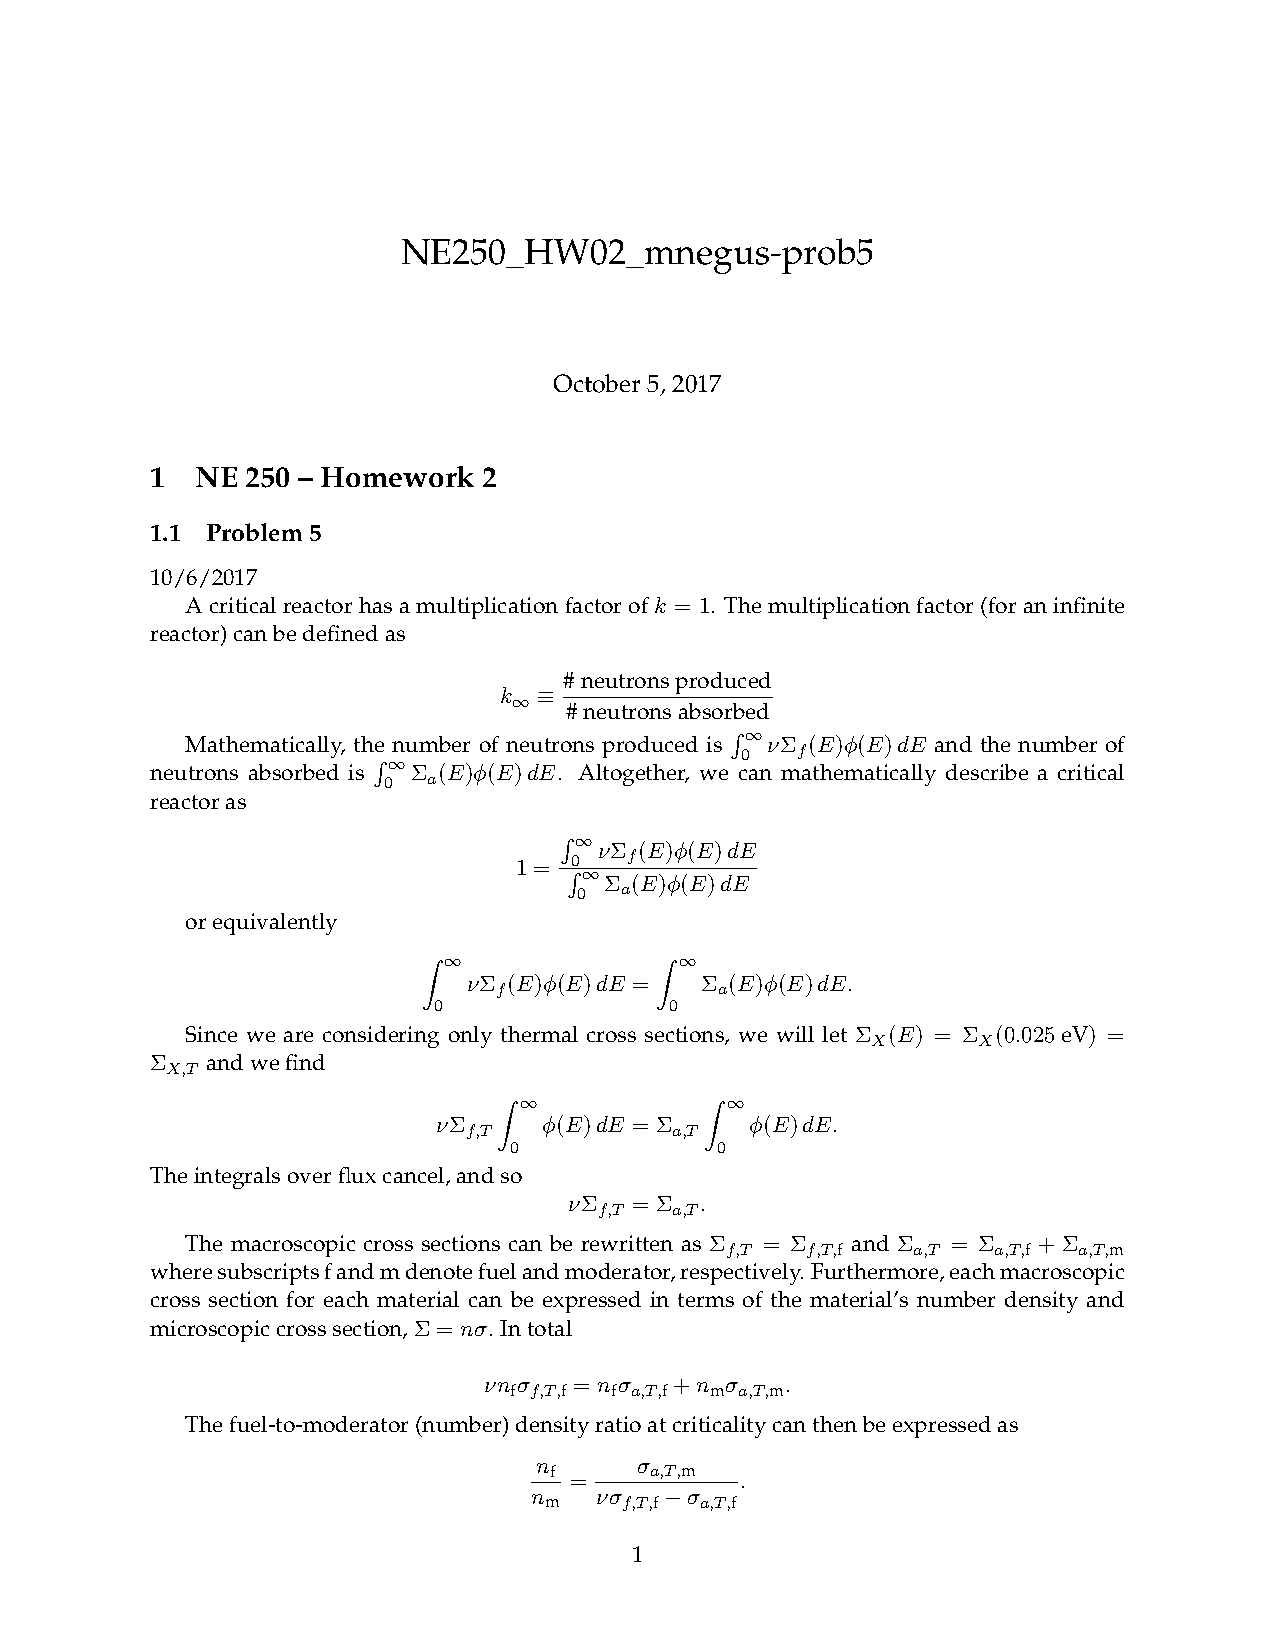
\includepdf[pages=-]{NE250_HW02_mnegus-prob5.pdf}
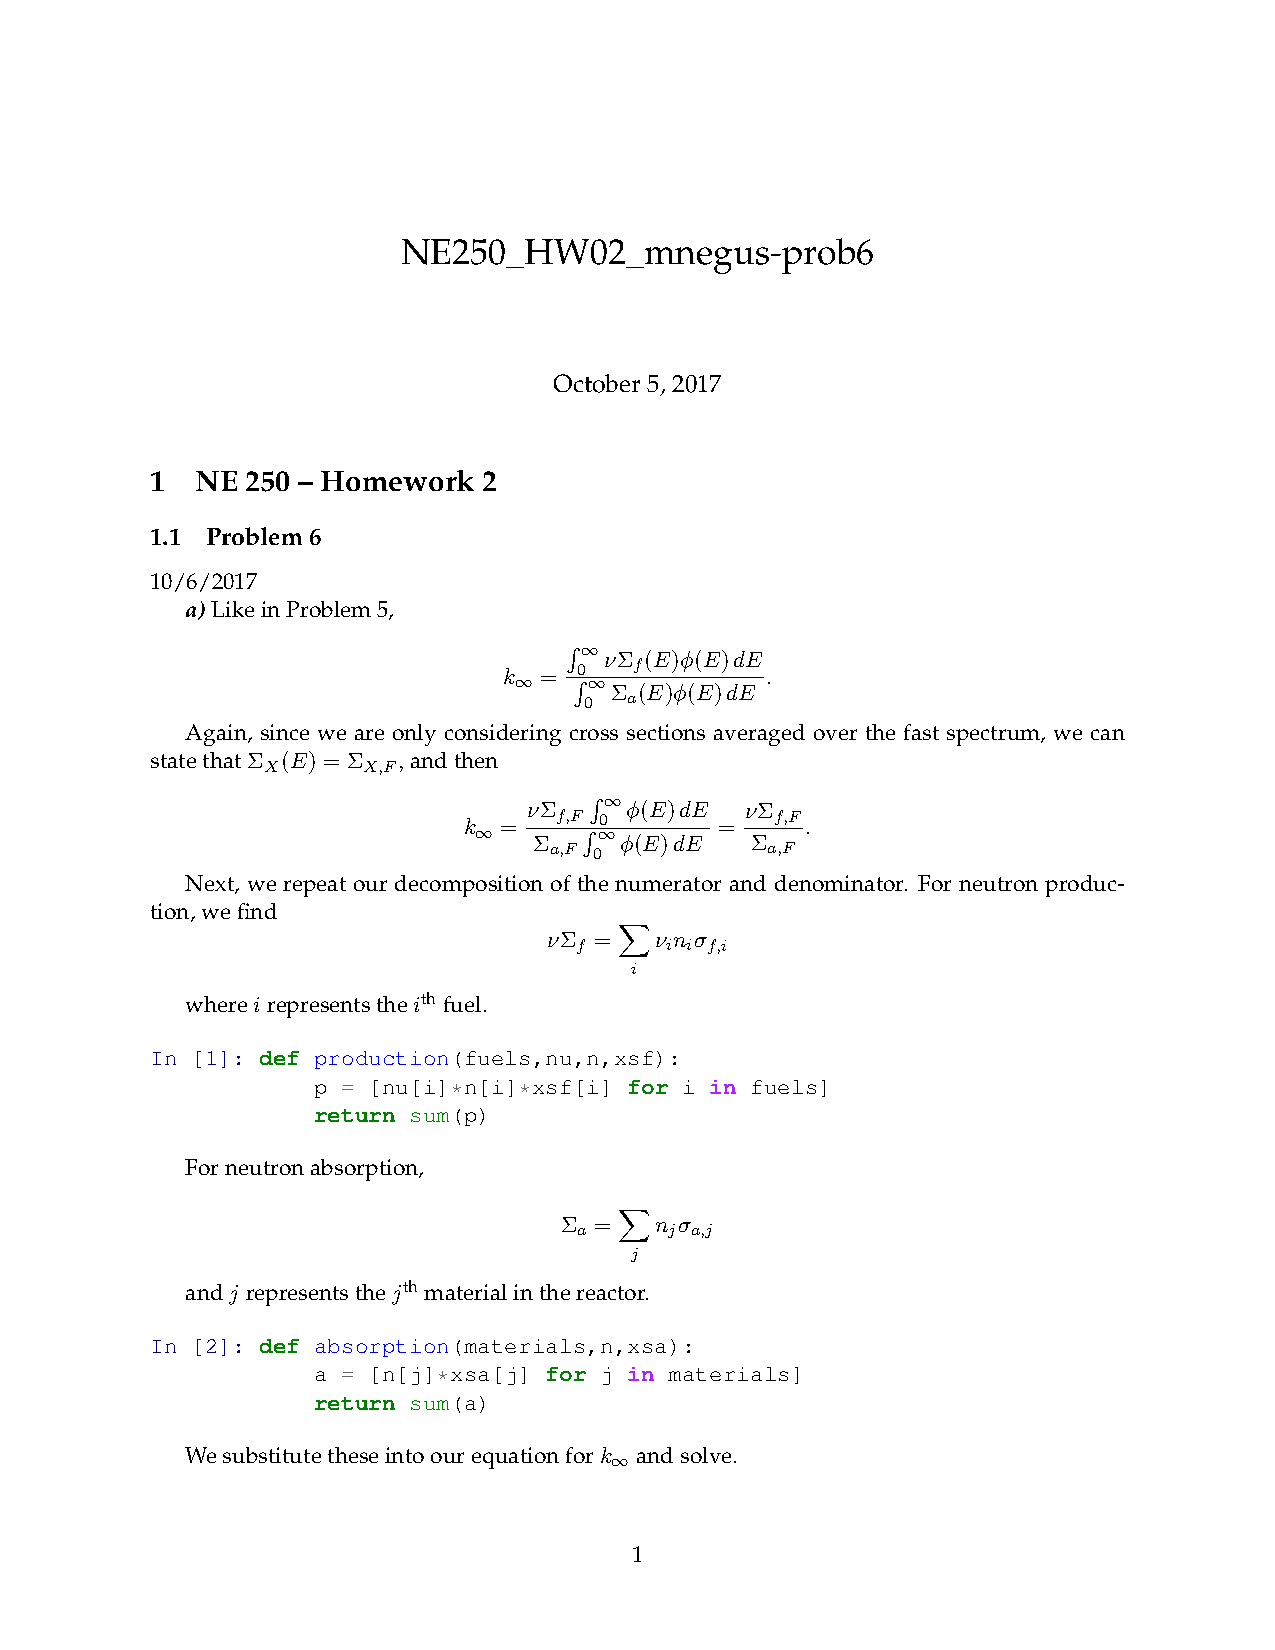
\includepdf[pages=-]{NE250_HW02_mnegus-prob6.pdf}

\end{document}







 
